\documentclass[10pt]{report}

% Paquetes y configuraciones adicionales
\usepackage{graphicx}
\usepackage[export]{adjustbox}
\usepackage{caption}
\usepackage{float}
\usepackage{titlesec}
\usepackage{geometry}
\usepackage{hyperref}
\usepackage{fontspec}

\setmainfont{Geist}



% Configura los márgenes
\geometry{
    left=2cm,   % Ajusta este valor al margen izquierdo deseado
    right=2cm,  % Ajusta este valor al margen derecho deseado
    top=3cm,
    bottom=3cm,
}

% Configuración de los títulos de las secciones
\titlespacing{\section}{0pt}{\parskip}{\parskip}
\titlespacing{\subsection}{0pt}{\parskip}{\parskip}
\titlespacing{\subsubsection}{0pt}{\parskip}{\parskip}


\begin{document}
	
	% Portada del informe
	
	\title{Disparadores y Vistas en SQL}
	\author{Samuel Martín Morales \texttt{alu0101359526@ull.edu.es} \and Jorge Domínguez González \texttt{alu0101330600@ull.edu.es}}
	\date{\today}
	
	\maketitle
	
	% Índice
	\tableofcontents
	
	% Secciones del informe
	\chapter{Introducción}
  Para esta cuarta práctica de la asignatura \emph{Administración y Diseño de Bases de Datos} se solicita el empleo de una base de datos que debe de ser restaurada de manera previa a la implementación de una serie de ejercicios que son demandados haciendo uso de dicha base de datos.
\\
	En este caso, la base de datos a emplear se denomina como \emph{\textbf{alquilerdvd.tar}} y se encuentra disponible en el campus virtual de la asignatura. Pero, puede ser descargada desde el siguiente enlace de \href{https://github.com/Samuelmm15/PostgreSQL-Rent/blob/main/AlquilerPractica.tar}{GitHub}.
\\
	Dicha base de datos se encuentra en formato \emph{.tar} por lo que, para poder restaurarla, se debe de emplear el siguiente comando:

	\begin{verbatim}
		$ pg_restore -U postgres -d alquilerdvd alquilerdvd.tar
	\end{verbatim}

	Es decir, el comando anterior restaura la base de datos \emph{alquilerdvd} haciendo uso del fichero \emph{alquilerdvd.tar} y empleando el usuario \emph{postgres}.
\\
	Una vez restaurada la base de datos, se puede proceder a la realización de los distintos ejercicios.
\\
	\chapter{Resultados}
	\section{Ejercicio 1}
	Para el primer ejercicio de la práctica, se deben de identificar las distintas tablas, vistas y secuencias que tiene la base de datos que ha sido restaurada.
\\
	Tras la carga de la base de datos a partir del fichero con extensión \emph{.tar}, se puede observar que la base de datos \emph{alquilerdvd} cuenta con un total de 15 tablas, 0 vistas y 15 secuencias. Para poder visualizar todos estos datos comentados sobre la base de datos, se hace uso de la terminal interactiva de \emph{PostgreSQL}, es decir, de \emph{psql}, y, una vez dentro de la base de datos se ejecutan los siguientes comandos para obtener los distintos valores obsevados anteriormente:

	\begin{verbatim}
		# \dt 		-- Muestra las tablas de la base de datos 
		# \dv		 -- Muestra las vistas de la base de datos
		# \ds		 -- Muestra las secuencias de la base de datos
	\end{verbatim}

	Para comprobar todo esto anterior se puede observar la siguiente imagen \ref{fig:Exercice-1}:

	\begin{figure}[H]
    \centering
    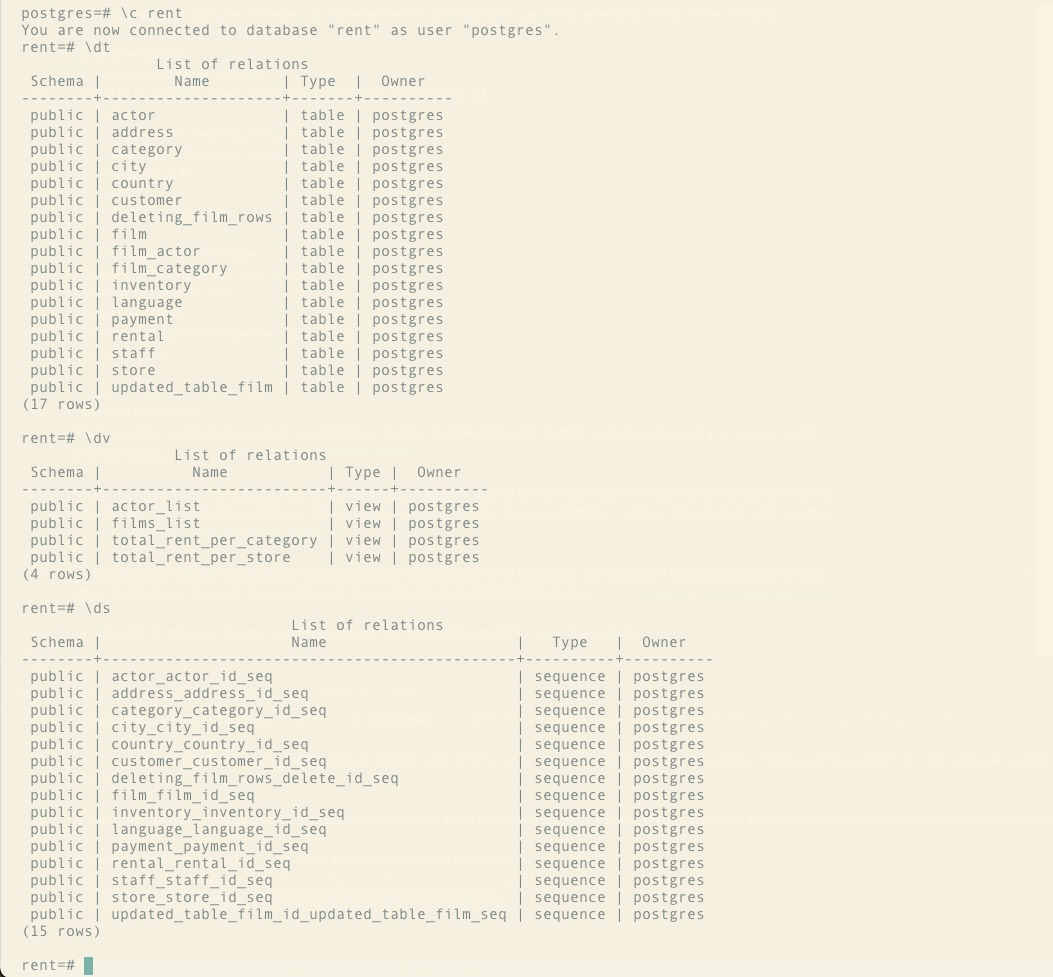
\includegraphics[scale=0.4]{img/Exercice-1-Comprobation.jpeg}
    \caption{Ejecución de los comandos dt, dv, ds en la terminal psql.}
    \label{fig:Exercice-1}
  \end{figure}

	\section{Ejercicio 2}
	Para el segundo ejercicio de la práctica, se solicita la identificación de las tablas más importantes de la base de datos junto con sus atributos y relaciones más relevantes entre las distintas tablas.
\\	
		\subsubsection{Tabla \texttt{film}}
		\begin{itemize}
		  \item Elementos Clave:
		  \begin{itemize}
			\item \texttt{film\_id}
			\item \texttt{title}
			\item \texttt{description}
			\item \texttt{category}
			\item \texttt{price}
			\item \texttt{length}
			\item \texttt{rating}
		  \end{itemize}
		  \item Descripción: Contiene información sobre las películas disponibles para alquiler, como su título, descripción, categoría, precio, duración y calificación.
		\end{itemize}
		
		\subsubsection{Tabla \texttt{actor}}
		\begin{itemize}
		  \item Elementos Clave:
		  \begin{itemize}
			\item \texttt{actor\_id}
			\item \texttt{first\_name}
			\item \texttt{last\_name}
		  \end{itemize}
		  \item Descripción: Almacena detalles sobre los actores que participan en las películas.
		\end{itemize}

		\subsubsection{Tabla \texttt{customer}}
		\begin{itemize}
		  \item Elementos Clave:
		  \begin{itemize}
			\item \texttt{customer\_id}
			\item \texttt{first\_name}
			\item \texttt{last\_name}
			\item \texttt{email}
			\item \texttt{address\_id}
		  \end{itemize}
		  \item Descripción: Registra información sobre los clientes que realizan alquileres, incluyendo sus nombres, correos electrónicos y direcciones.
		\end{itemize}
		
		\subsubsection{Tabla \texttt{rental}}
		\begin{itemize}
		  \item Elementos Clave:
		  \begin{itemize}
			\item \texttt{rental\_id}
			\item \texttt{rental\_date}
			\item \texttt{return\_date}
			\item \texttt{customer\_id}
			\item \texttt{inventory\_id}
		  \end{itemize}
		  \item Descripción: Realiza un seguimiento de los alquileres, incluyendo la fecha de alquiler, la fecha de devolución y los clientes involucrados.
		\end{itemize}
		
		\subsubsection{Tabla \texttt{inventory}}
		\begin{itemize}
		  \item Elementos Clave:
		  \begin{itemize}
			\item \texttt{inventory\_id}
			\item \texttt{film\_id}
			\item \texttt{store\_id}
		  \end{itemize}
		  \item Descripción: Administra el inventario de películas disponible en las tiendas.
		\end{itemize}
		
		\subsubsection{Tabla \texttt{store}}
		\begin{itemize}
		  \item Elementos Clave:
		  \begin{itemize}
			\item \texttt{store\_id}
			\item \texttt{manager\_staff\_id}
			\item \texttt{address\_id}
		  \end{itemize}
		  \item Descripción: Contiene información sobre las tiendas, como el personal encargado y la dirección.
		\end{itemize}
		
		\subsubsection{Tabla \texttt{payment}}
		\begin{itemize}
		  \item Elementos Clave:
		  \begin{itemize}
			\item \texttt{payment\_id}
			\item \texttt{customer\_id}
			\item \texttt{amount}
			\item \texttt{payment\_date}
		  \end{itemize}
		  \item Descripción: Registra los pagos realizados por los clientes por los alquileres de películas.
		\end{itemize}
	
	\section{Ejercicio 3}
	Tras la identificación de las distintas tablas más importantes de la base de datos junto con sus atributos  y relaciones entre las distintas tablas, se procede a la implementación de distintas consultas que permitan obtener aquella información que es solicitada en el enunciado del ejercicio.
\\
	\subsection{Ventas totales}
	Para obtener las ventas totales por categoría de películas ordendas de manera descendente, se emplea la siguiente consulta:

	\begin{verbatim}
		SELECT COUNT(*) AS total_rent, category.name AS category_name
		FROM rental
		INNER JOIN inventory ON rental.inventory_id = inventory.inventory_id
		INNER JOIN film ON inventory.film_id = film.film_id
		INNER JOIN film_category ON film.film_id = film_category.film_id
		INNER JOIN category ON film_category.category_id = category.category_id
		GROUP BY category_name
		ORDER BY total_rent DESC;
	\end{verbatim}

	Resultado de la consulta anterior \ref{fig:Exercice-2-1}:

	\begin{figure}[H]
		\centering
		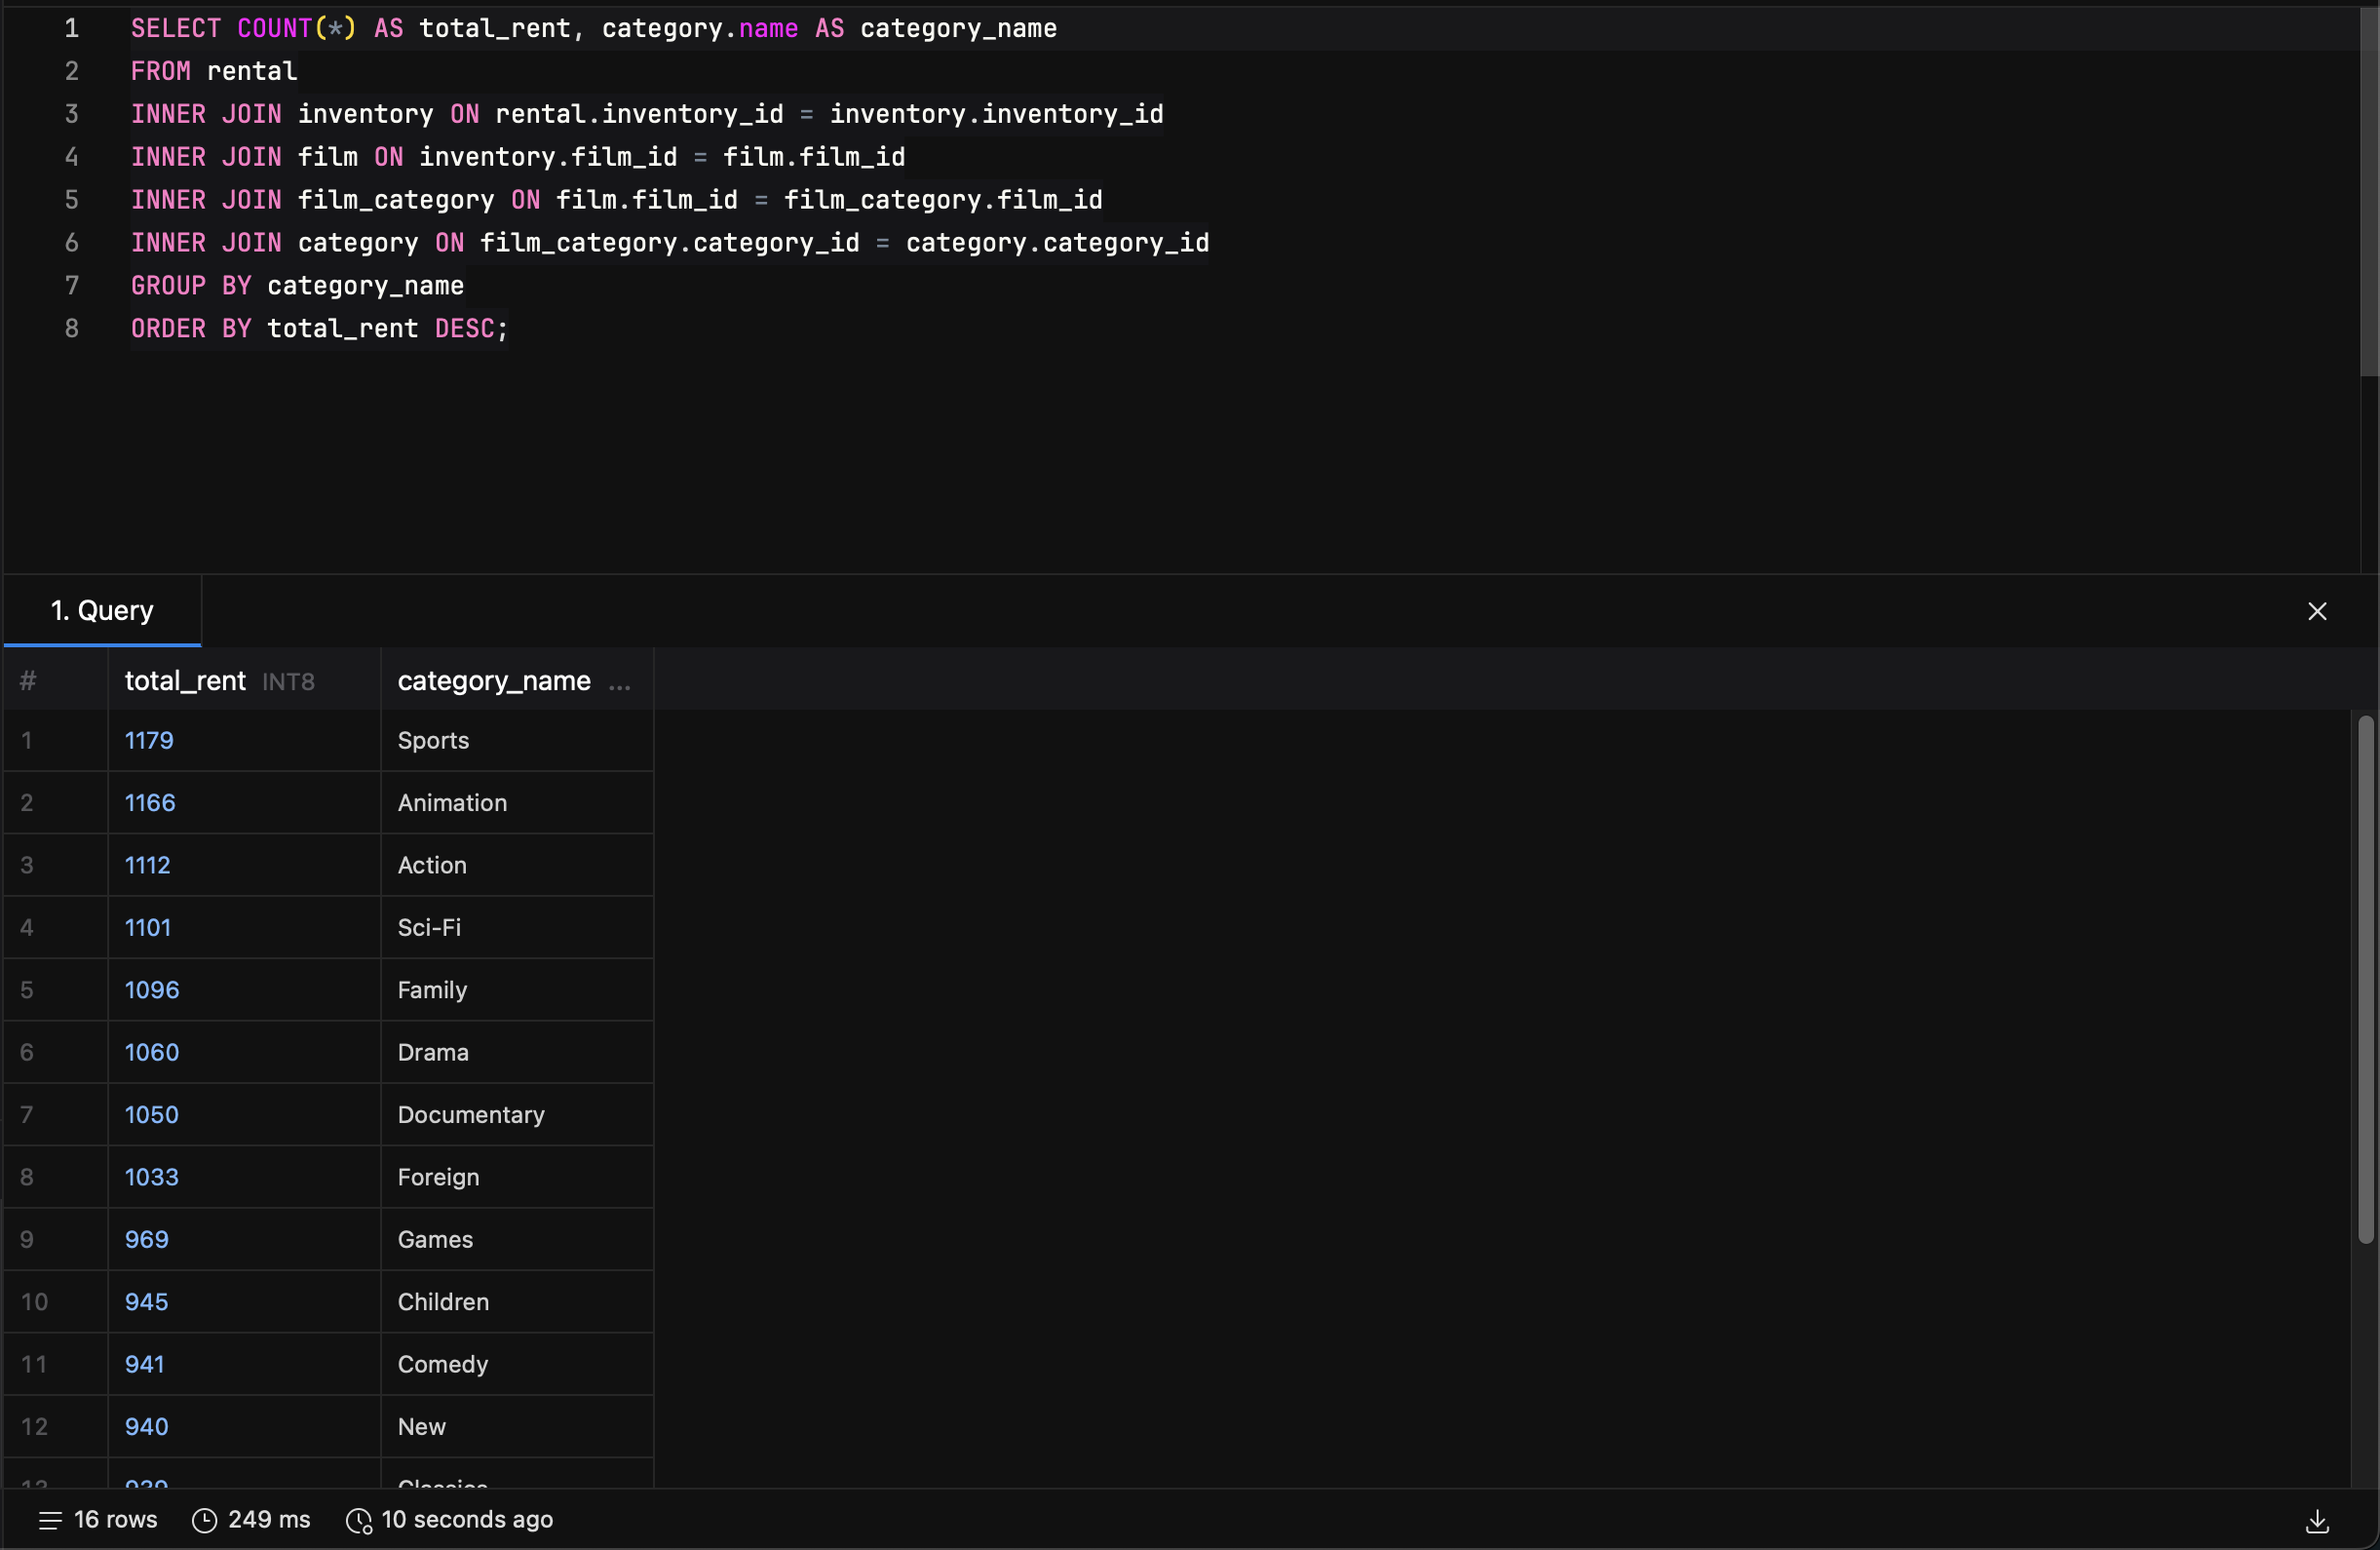
\includegraphics[scale=0.5]{img/Exercice-2.2.1-Comprobation.png}
		\caption{Resultado de la consulta de las ventas totales por categoría.}
		\label{fig:Exercice-2-1}
	\end{figure}

	\subsection{Ventas totales por tienda}
	Para obtener las ventas totales por tienda donde se refleja la ciudad, el país y el encargado,  se emplea la siguiente consulta:

	\begin{verbatim}
		SELECT COUNT(*) AS total_rent , store.store_id AS store_id, city.city || ', ' || country.country AS cityu_and_country, staff.first_name AS manager_staff_first_name, staff.last_name AS manager_staff_last_name
	FROM rental
	INNER JOIN inventory on rental.inventory_id = inventory.inventory_id
	INNER JOIN store ON inventory.store_id = store.store_id
	INNER JOIN staff ON store.manager_staff_id = staff.staff_id
	INNER JOIN address ON store.address_id = address.address_id
	INNER JOIN city ON address.city_id = city.city_id
	INNER JOIN country ON city.country_id = country.country_id
	GROUP BY store.store_id, manager_staff_first_name, manager_staff_last_name, city, country
	ORDER BY total_rent DESC;
	\end{verbatim}

	Resultado de la consulta anterior \ref{fig:Exercice-2-2}:

	\begin{figure}[H]
		\centering
		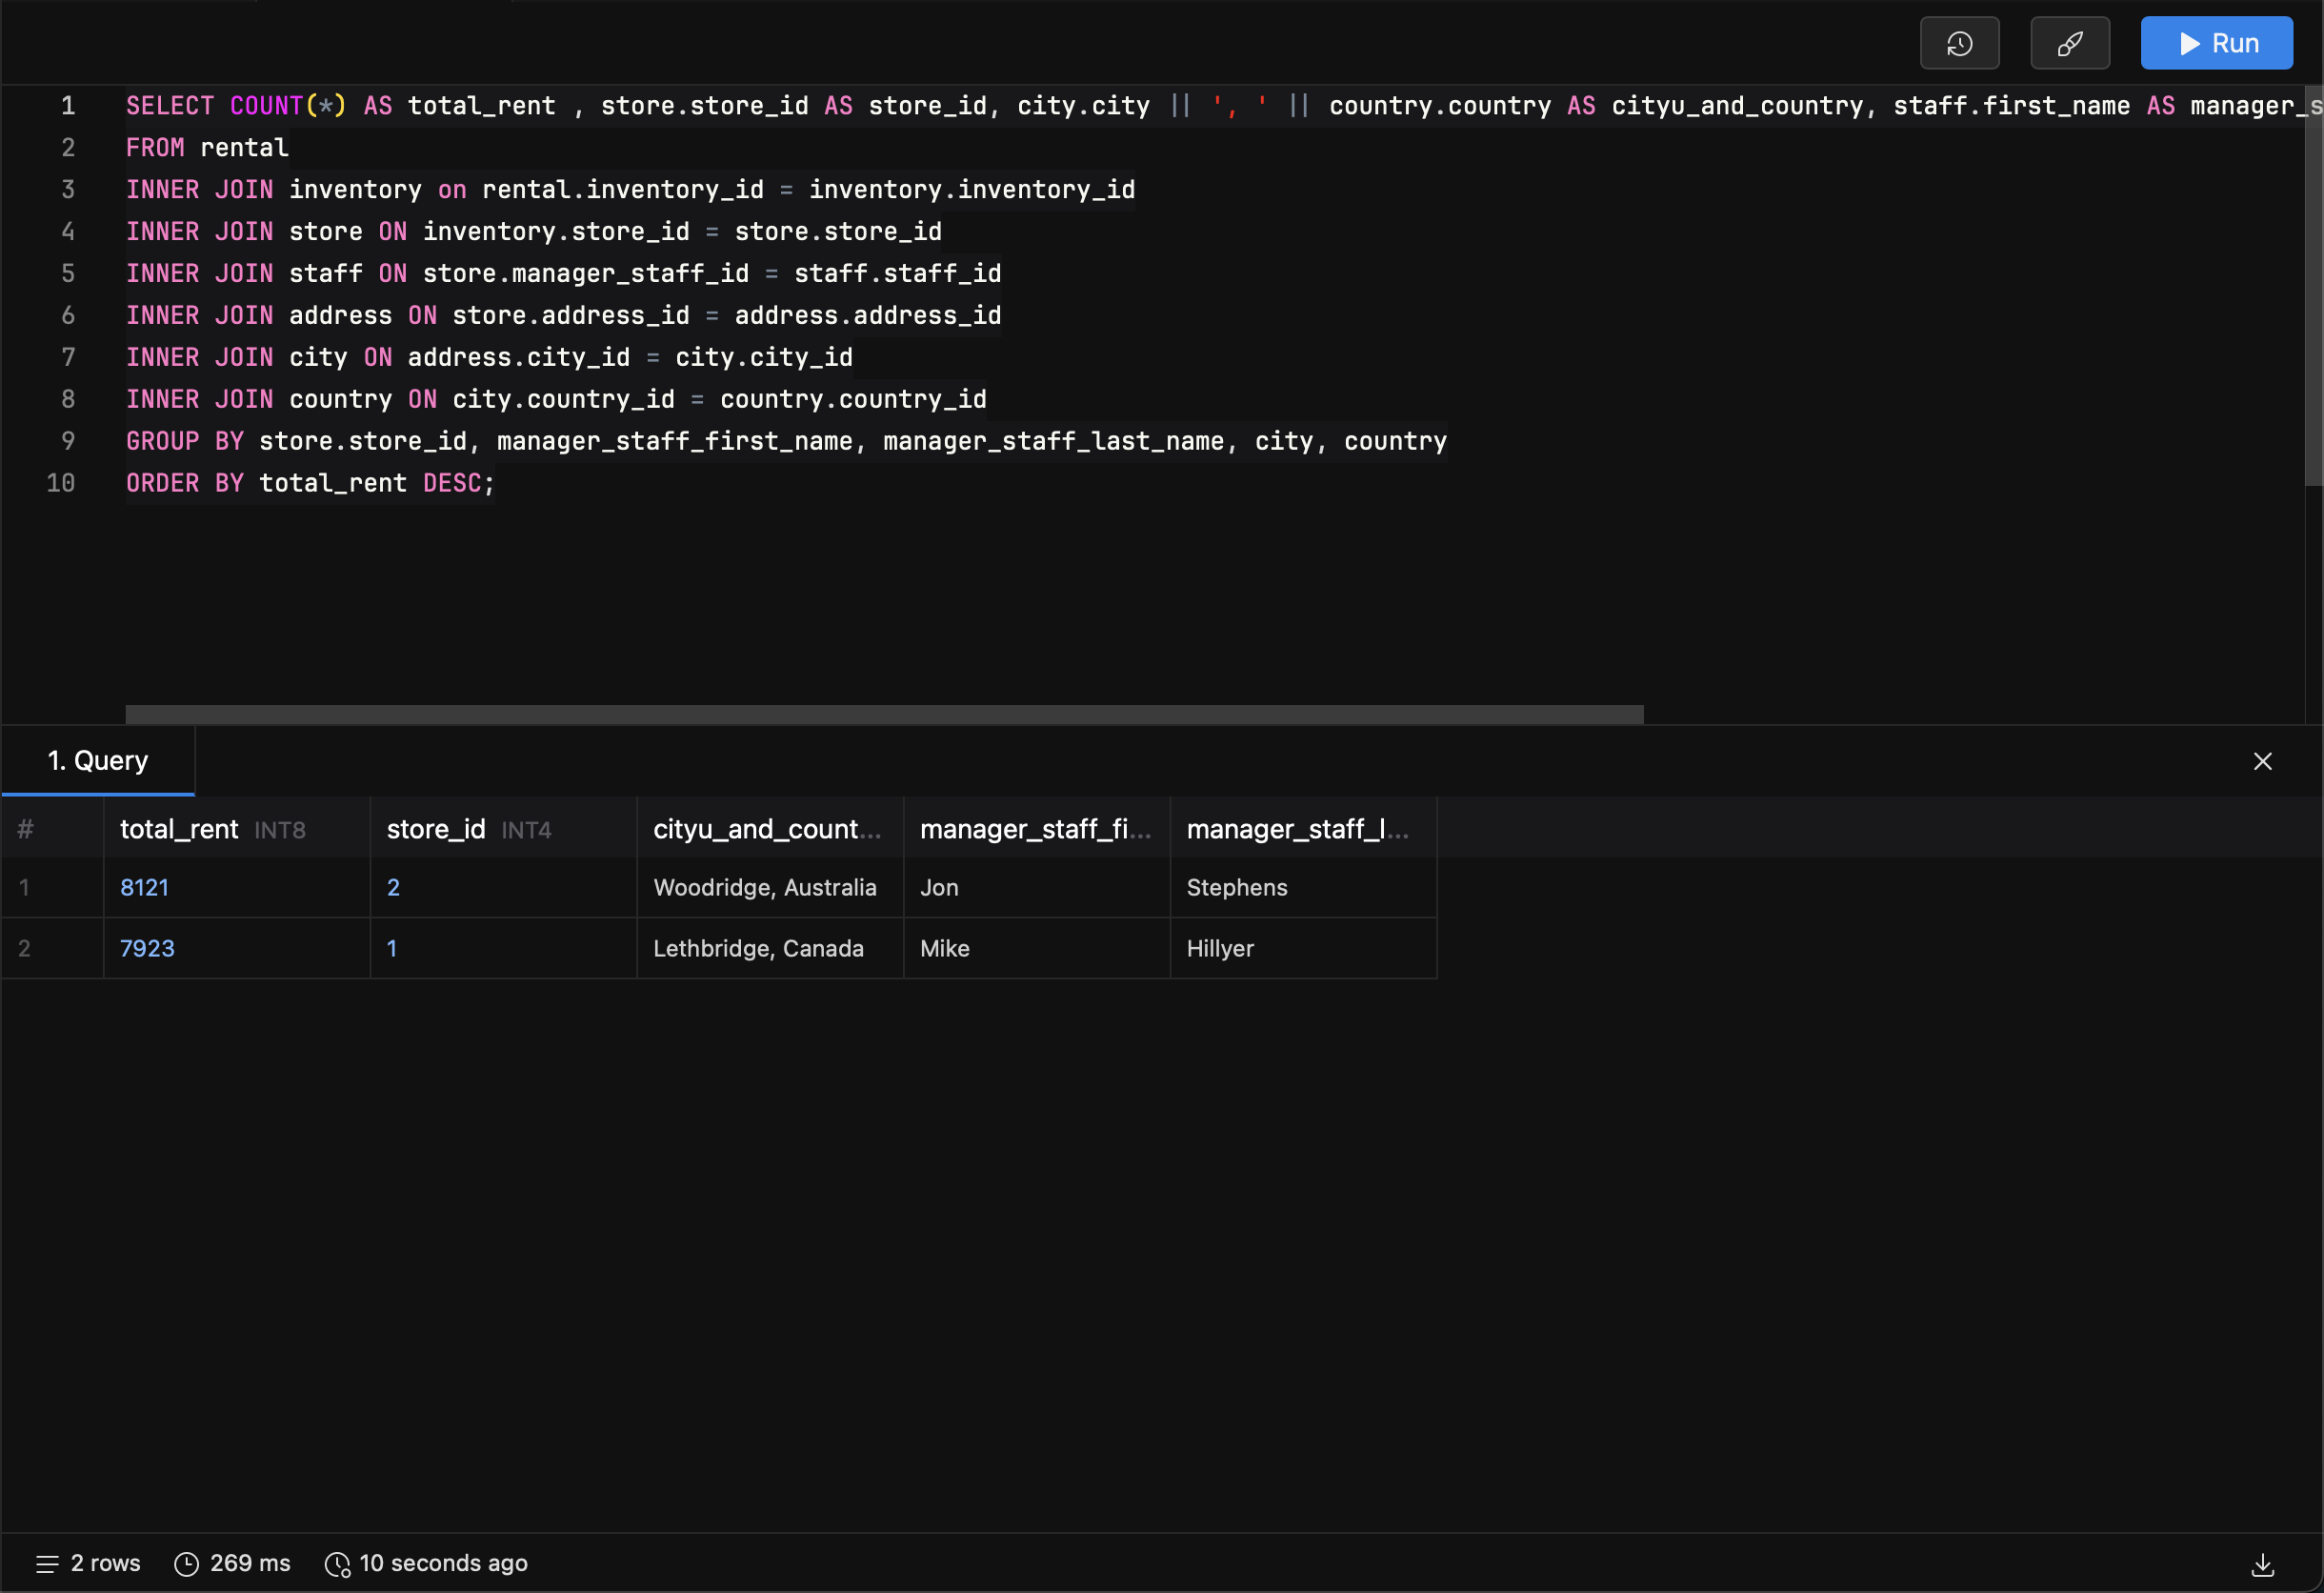
\includegraphics[scale=0.5]{img/Exercice-2.2.2-Comprobation.png}
		\caption{Resultado de la consulta de las ventas totales por tienda.}
		\label{fig:Exercice-2-2}
	\end{figure}

	\fbox{\parbox{\textwidth}{
    \textbf{Nota:} para la consulta anterior se ha empleado una concatenación de cadenas de caracteres para poder obtener la ciudad y el país en una misma columna, para ello, se ha hecho uso de la doble barra vertical  que permite establecer la concatenación por pares de elementos, y para el ejemplo de consulta observado anteriormente, se hace uso del separador \emph{","} para realizar esta operación.
}}
\\
	
	\subsection{Lista de películas}
	Para obtener una lista de películas junto con sus actores, se emplea la siguiente consulta:

	\begin{verbatim}
		SELECT film.film_id, title, description, category.name AS category_name,rental_rate, length, rating ,actor.first_name || '  ' || actor.last_name AS actor_name
		FROM film
		INNER JOIN film_actor ON film.film_id = film_actor.film_id
		INNER JOIN actor ON film_actor.actor_id = actor.actor_id
		INNER JOIN film_category ON film.film_id = film_category.film_id
		INNER JOIN category ON film_category.category_id = category.category_id
		ORDER BY film_id;
	\end{verbatim}

	Resultado de la consulta anterior \ref{fig:Exercice-2-3}:

	\begin{figure}[H]
		\centering
		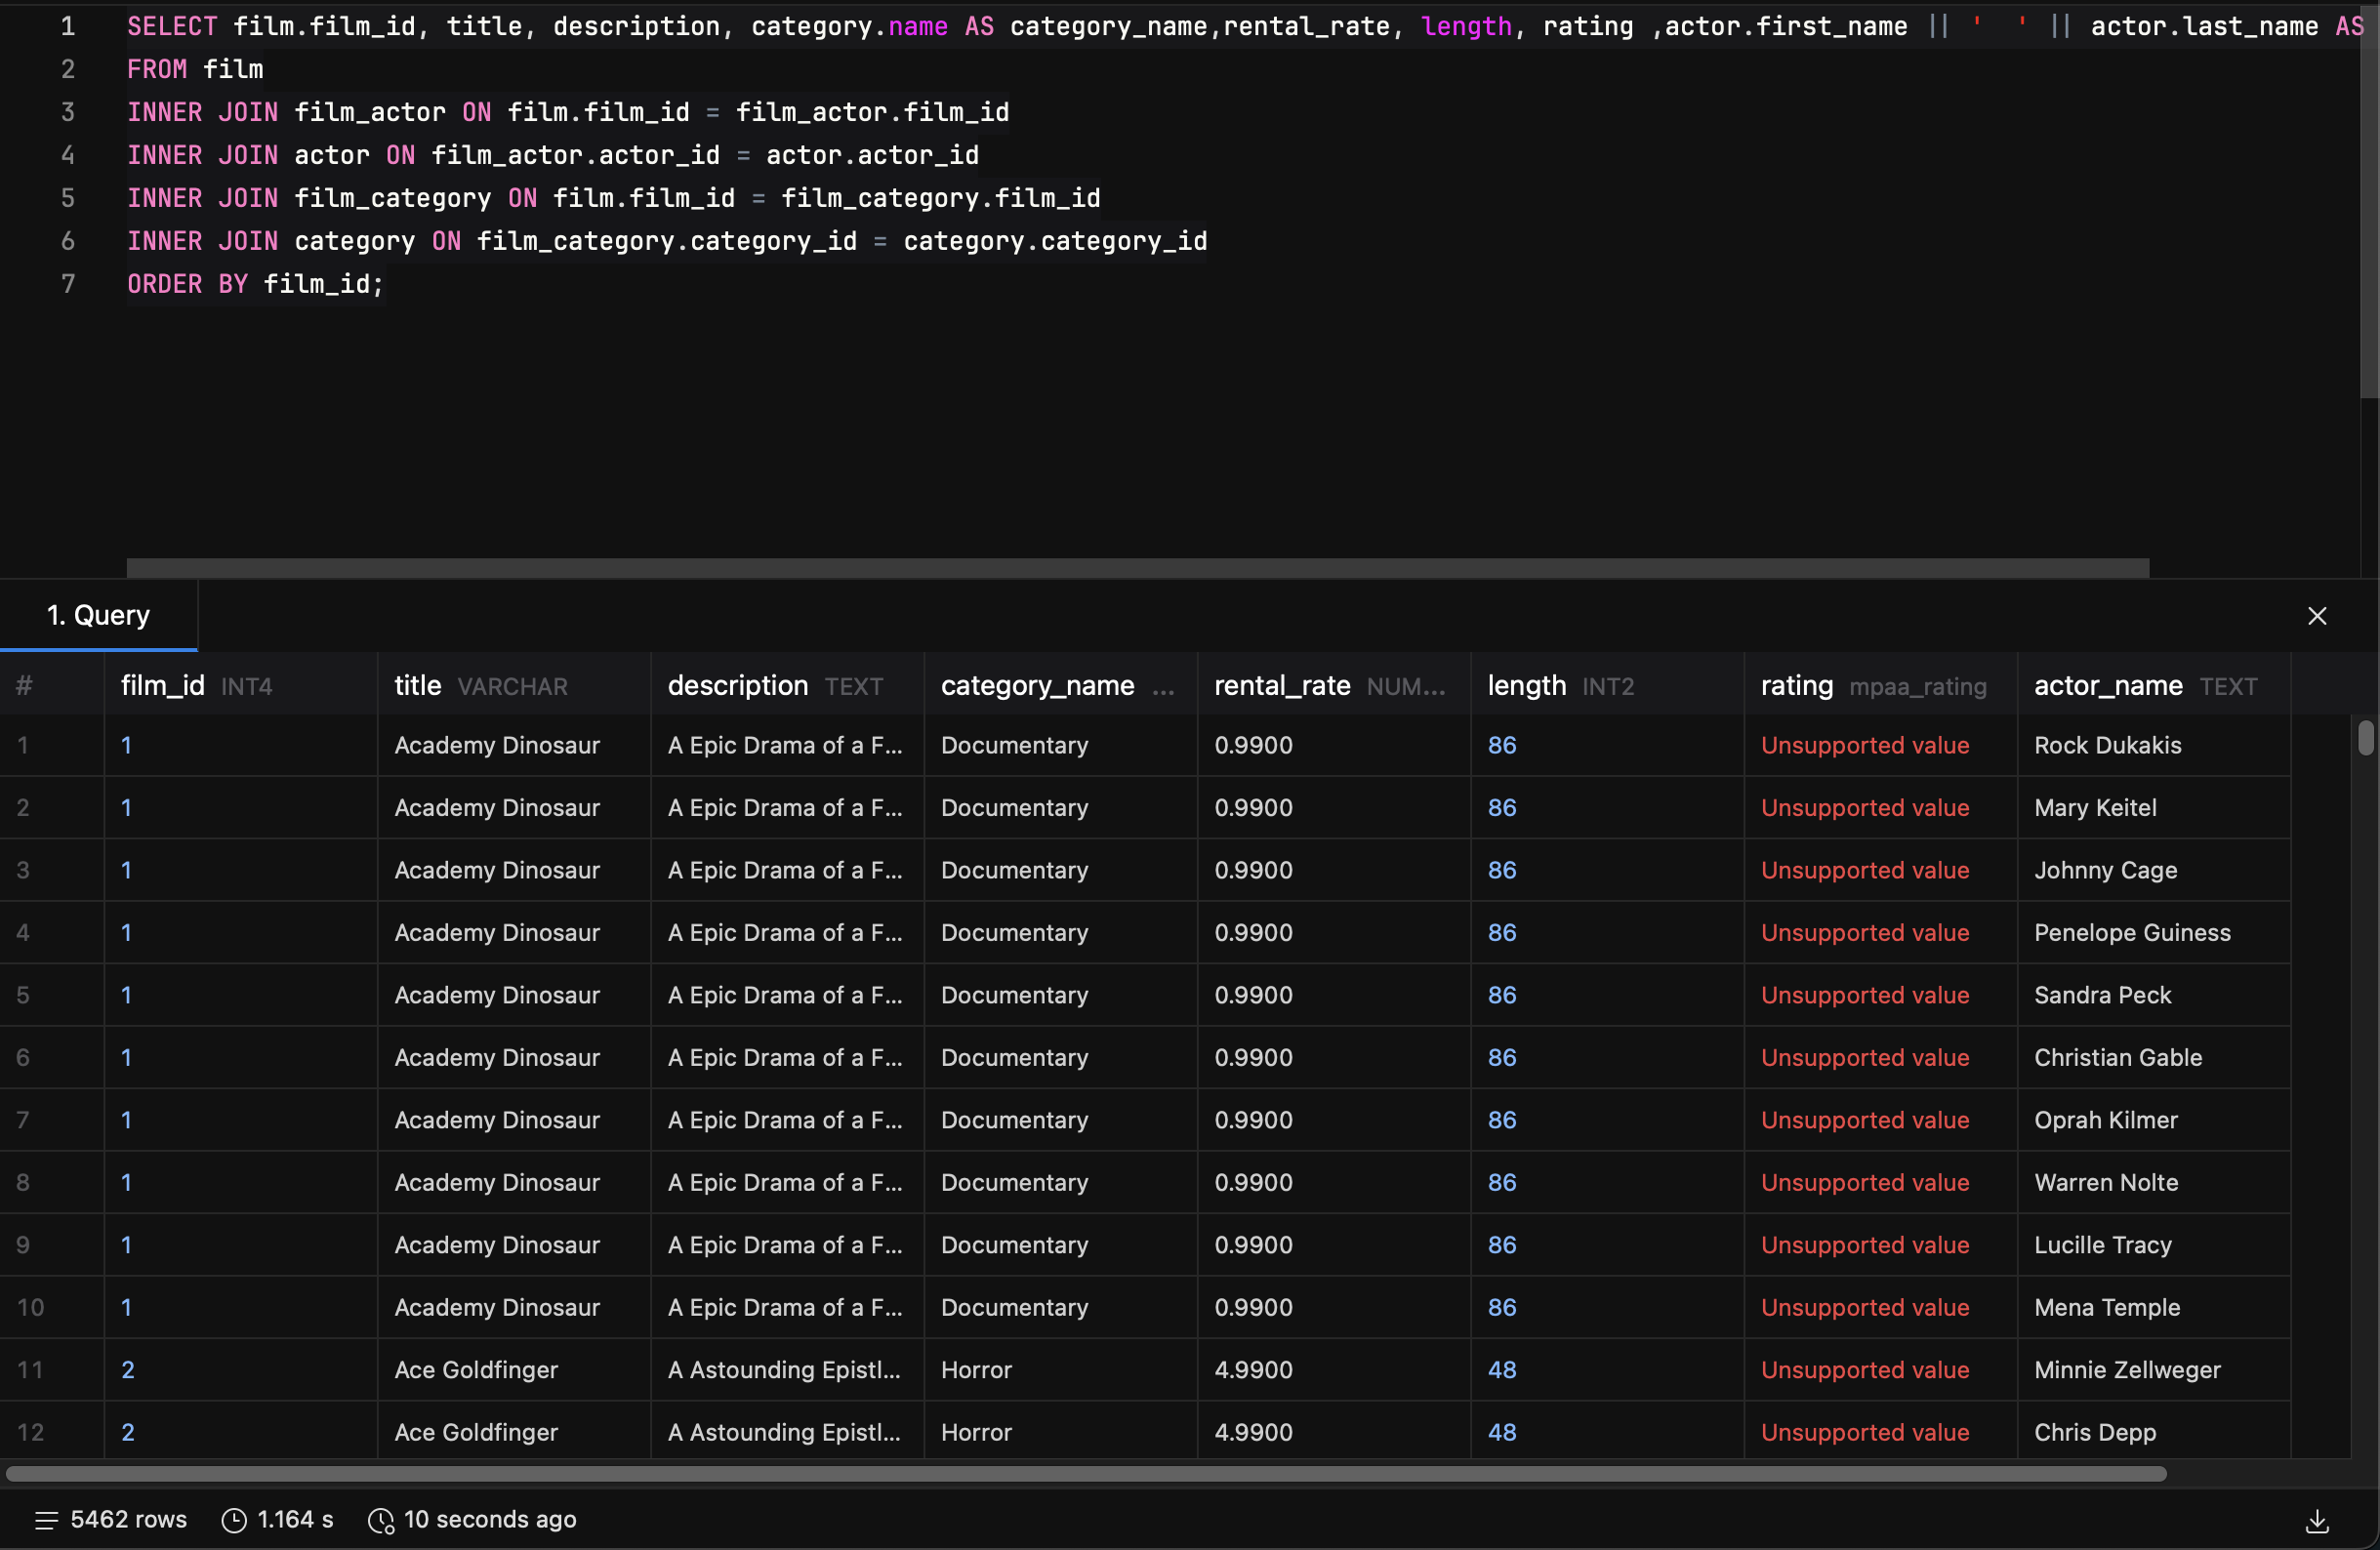
\includegraphics[scale=0.5]{img/Exercice-2.2.3-Comprobation.png}
		\caption{Resultado de la consulta de la lista de películas.}
		\label{fig:Exercice-2-3}
	\end{figure}

	\subsection{información de los actores}
	Para obtener información de los distintos actores junto con sus películas existentes en la base de datos, se implementa la siguiente consulta:

	\begin{verbatim}
		SELECT actor.actor_id, actor.first_name, actor.last_name,film.title || ' : ' || film.description || ' : ' || category.name AS films_made
		FROM actor
		INNER JOIN film_actor ON actor.actor_id = film_actor.actor_id
		INNER JOIN film ON film_actor.film_id = film.film_id
		INNER JOIN film_category ON film.film_id = film_category.film_id
		INNER JOIN category ON film_category.category_id = category.category_id
		GROUP BY actor.actor_id, actor.first_name, actor.last_name, films_made
		ORDER BY actor.actor_id;
	\end{verbatim}

	Resultado de la consulta anterior \ref{fig:Exercice-2-4}:

	\begin{figure}[H]
		\centering
		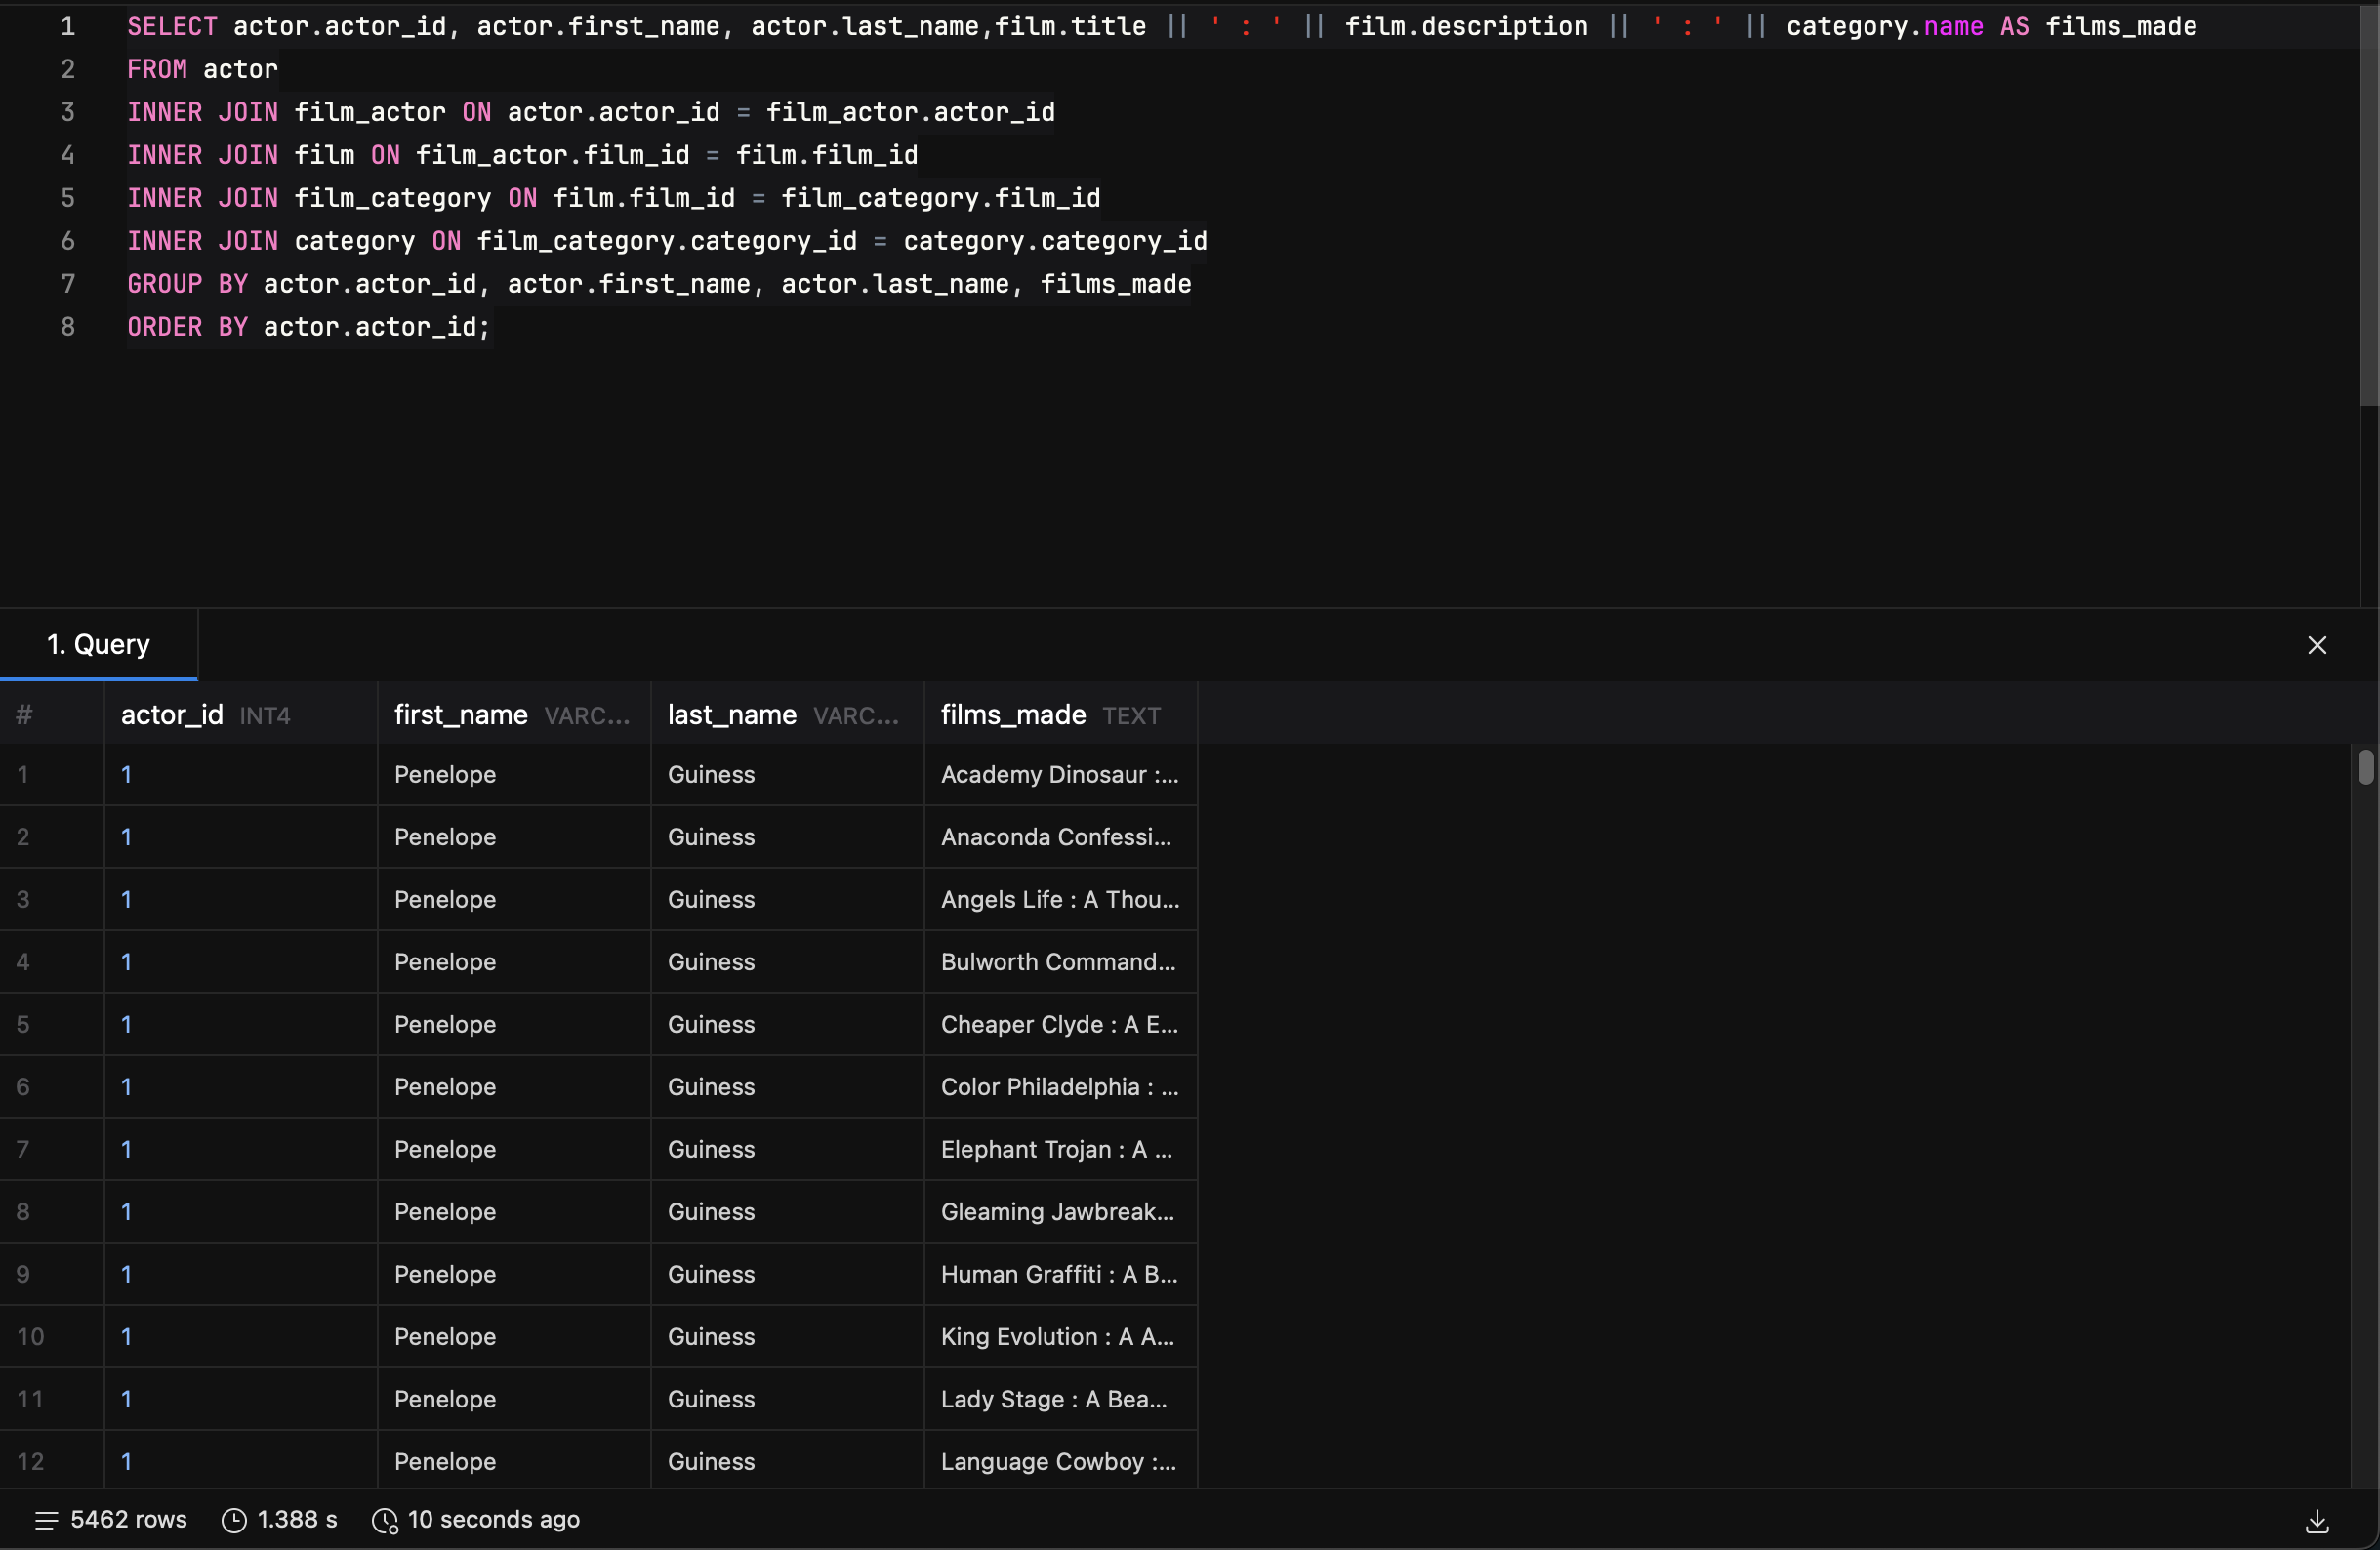
\includegraphics[scale=0.5]{img/Exercice-2.2.4-Comprobation.png}
		\caption{Resultado de la consulta de la información de los actores.}
		\label{fig:Exercice-2-4}
	\end{figure}

	\section{Ejercicio 4}
	Implementación de todas las vistas a partir de las consultas realizadas en el ejercicio anterior.
\\
	\subsection{Vista 1: Ventas totales}
	Para la implementación de la primera vista, se emplea la siguiente consulta:

	\begin{verbatim}
		CREATE VIEW total_rent_per_category AS
		SELECT COUNT(*) AS total_rent, category.name AS category_name
		FROM rental
		INNER JOIN inventory ON rental.inventory_id = inventory.inventory_id
		INNER JOIN film ON inventory.film_id = film.film_id
		INNER JOIN film_category ON film.film_id = film_category.film_id
		INNER JOIN category ON film_category.category_id = category.category_id
		GROUP BY category_name
		ORDER BY total_rent DESC;
	\end{verbatim}
	
	\subsection{Vista 2: Ventas totales por tienda}
	Para la implementación de la segunda vista, se emplea la siguiente consulta:

	\begin{verbatim}
		CREATE VIEW total_rent_per_store AS
		SELECT COUNT(*) AS total_rent , store.store_id AS store_id, city.city || ', ' || country.country AS cityu_and_country, staff.first_name AS manager_staff_first_name, staff.last_name AS manager_staff_last_name
		FROM rental
		INNER JOIN inventory on rental.inventory_id = inventory.inventory_id
		INNER JOIN store ON inventory.store_id = store.store_id
		INNER JOIN staff ON store.manager_staff_id = staff.staff_id
		INNER JOIN address ON store.address_id = address.address_id
		INNER JOIN city ON address.city_id = city.city_id
		INNER JOIN country ON city.country_id = country.country_id
		GROUP BY store.store_id, manager_staff_first_name, manager_staff_last_name, city, country
		ORDER BY total_rent DESC;
	\end{verbatim}

	\subsection{Vista 3: Lista de películas}
	Para la implementación de la tercera vista, se emplea la siguiente consulta:

	\begin{verbatim}
		CREATE VIEW films_list AS
		SELECT film.film_id, title, description, category.name AS category_name,rental_rate, length, rating ,actor.first_name || '  ' || actor.last_name AS actor_name
		FROM film
		INNER JOIN film_actor ON film.film_id = film_actor.film_id
		INNER JOIN actor ON film_actor.actor_id = actor.actor_id
		INNER JOIN film_category ON film.film_id = film_category.film_id
		INNER JOIN category ON film_category.category_id = category.category_id
		ORDER BY film_id;
	\end{verbatim}

	\subsection{Vista 4: Información de los actores}
	Para la implementación de la cuarta vista, se emplea la siguiente consulta:

	\begin{verbatim}
		CREATE VIEW actor_list AS
		SELECT actor.actor_id, actor.first_name, actor.last_name,film.title || ' : ' || film.description || ' : ' || category.name AS films_made
		FROM actor
		INNER JOIN film_actor ON actor.actor_id = film_actor.actor_id
		INNER JOIN film ON film_actor.film_id = film.film_id
		INNER JOIN film_category ON film.film_id = film_category.film_id
		INNER JOIN category ON film_category.category_id = category.category_id
		GROUP BY actor.actor_id, actor.first_name, actor.last_name, films_made
		ORDER BY actor.actor_id;
	\end{verbatim}

	\section{Ejercicio 5}
	Dentro del modelo de la base de datos \emph{alquilerdvd} se puede observar que existen tablas que emplean atributos que hacen uso de identificadores de tuplas que se encuentran dentro de otras tablas, es por ello, que para dichas tablas que emplean campos o columnas que hacen uso de  números de indentificación, se podrían implementar restricciones \emph{CHECK} que se encargen de comprobar que dichos números de identificación que son introducidos para las distintas tuplas,  corresponden con los números de identificación de las tablas a las que hacen referencia.

	Para poder comprender el tipo de restricción \emph{CHECK} que se puede implementar, se observa a continuación un ejemplo de posible implementación de restricción para aquellas tablas comentadas como ejemplo en el párrafo anterior:

	\begin{verbatim}
		ALTER TABLE payment
		ADD CONSTRAINT CK_ID_Cliente CHECK (customer_id IN (SELECT customer_id FROM customer));
	\end{verbatim}

	\section{Ejercicio 6}
	Para el quinto ejercicio de la práctica, se solicita la explicación del funcionamiento del trigger adjunto a continuación:

	\begin{verbatim}
		last_updated BEFORE UPDATE ON customer FOR EACH ROW EXECUTE
			PROCEDURE last_updated()
	\end{verbatim}

	El trigger representado anteriormente se activa o se ejecuta antes de que se actualice un registro de la tabla \emph{customer}, dónde, de manera previa a la actualización de cualquiera de los registros de la tabla \emph{customer}, se ejecuta la función \emph{last\_updated()}.
\\
	Teniendo en cuenta todo lo mencionado anteriormente, se puede observar que en la tabla \emph{film} se hace uso de un trigger que se ejecuta de manera previa a la insersión o la actualización de alguno de los registros de dicha tabla, es por ello que dicho disparador puede ser tomado como ejemplo de una tabla que haga uso de una solución similar a la que se ha mencionado anteriormente. Esto comentado puede ser observado en el bloque de código ajunto a continuación:

	\begin{verbatim}
		CREATE TRIGGER film_fulltext_trigger BEFORE INSERT OR UPDATE ON public.film FOR EACH ROW EXECUTE FUNCTION tsvector_update_trigger('fulltext', 'pg_catalog.english', 'title', 'description');
	\end{verbatim}

	\section{Ejercicio 7}
	Para el sexto ejercicio solicitado, se debe de contruir un disparador que se encargue de guardar en una nueva tabla creada la fecha de cuando se insertó un nuevo registro dentro de la tabla \emph{film}.
\\
	Cabe destacar que para la implementación de dicho disparador se ha creado de manera previa una nueva tabla denominada como \emph{updated-table-film}, la cual tiene la siguiente estructura:

	\begin{verbatim}
		CREATE TABLE updated_table_film (
				id_updated_table_film SERIAL PRIMARY KEY,
				last_update TIMESTAMP NOT NULL
		);
	\end{verbatim}

	Una vez creada la tabla, se procede a la implementación del disparador, para ello se emplea la siguiente consulta:

	\begin{verbatim}
		-- First we create the function
		CREATE FUNCTION delete_table_film() RETURNS TRIGGER AS $$
				BEGIN
						INSERT INTO updated_table_film (last_update) VALUES (NOW());
						RETURN NEW;
				END;
		$$ LANGUAGE plpgsql;

		-- Then we create the trigger
		CREATE TRIGGER trigger_delete_table_film
		AFTER INSERT ON film
		FOR EACH ROW
		EXECUTE FUNCTION delete_table_film();
	\end{verbatim}

	Comprobación del funcionamiento del disparador \ref{fig:Exercice-6}:

	\begin{figure}[H]
		\centering
		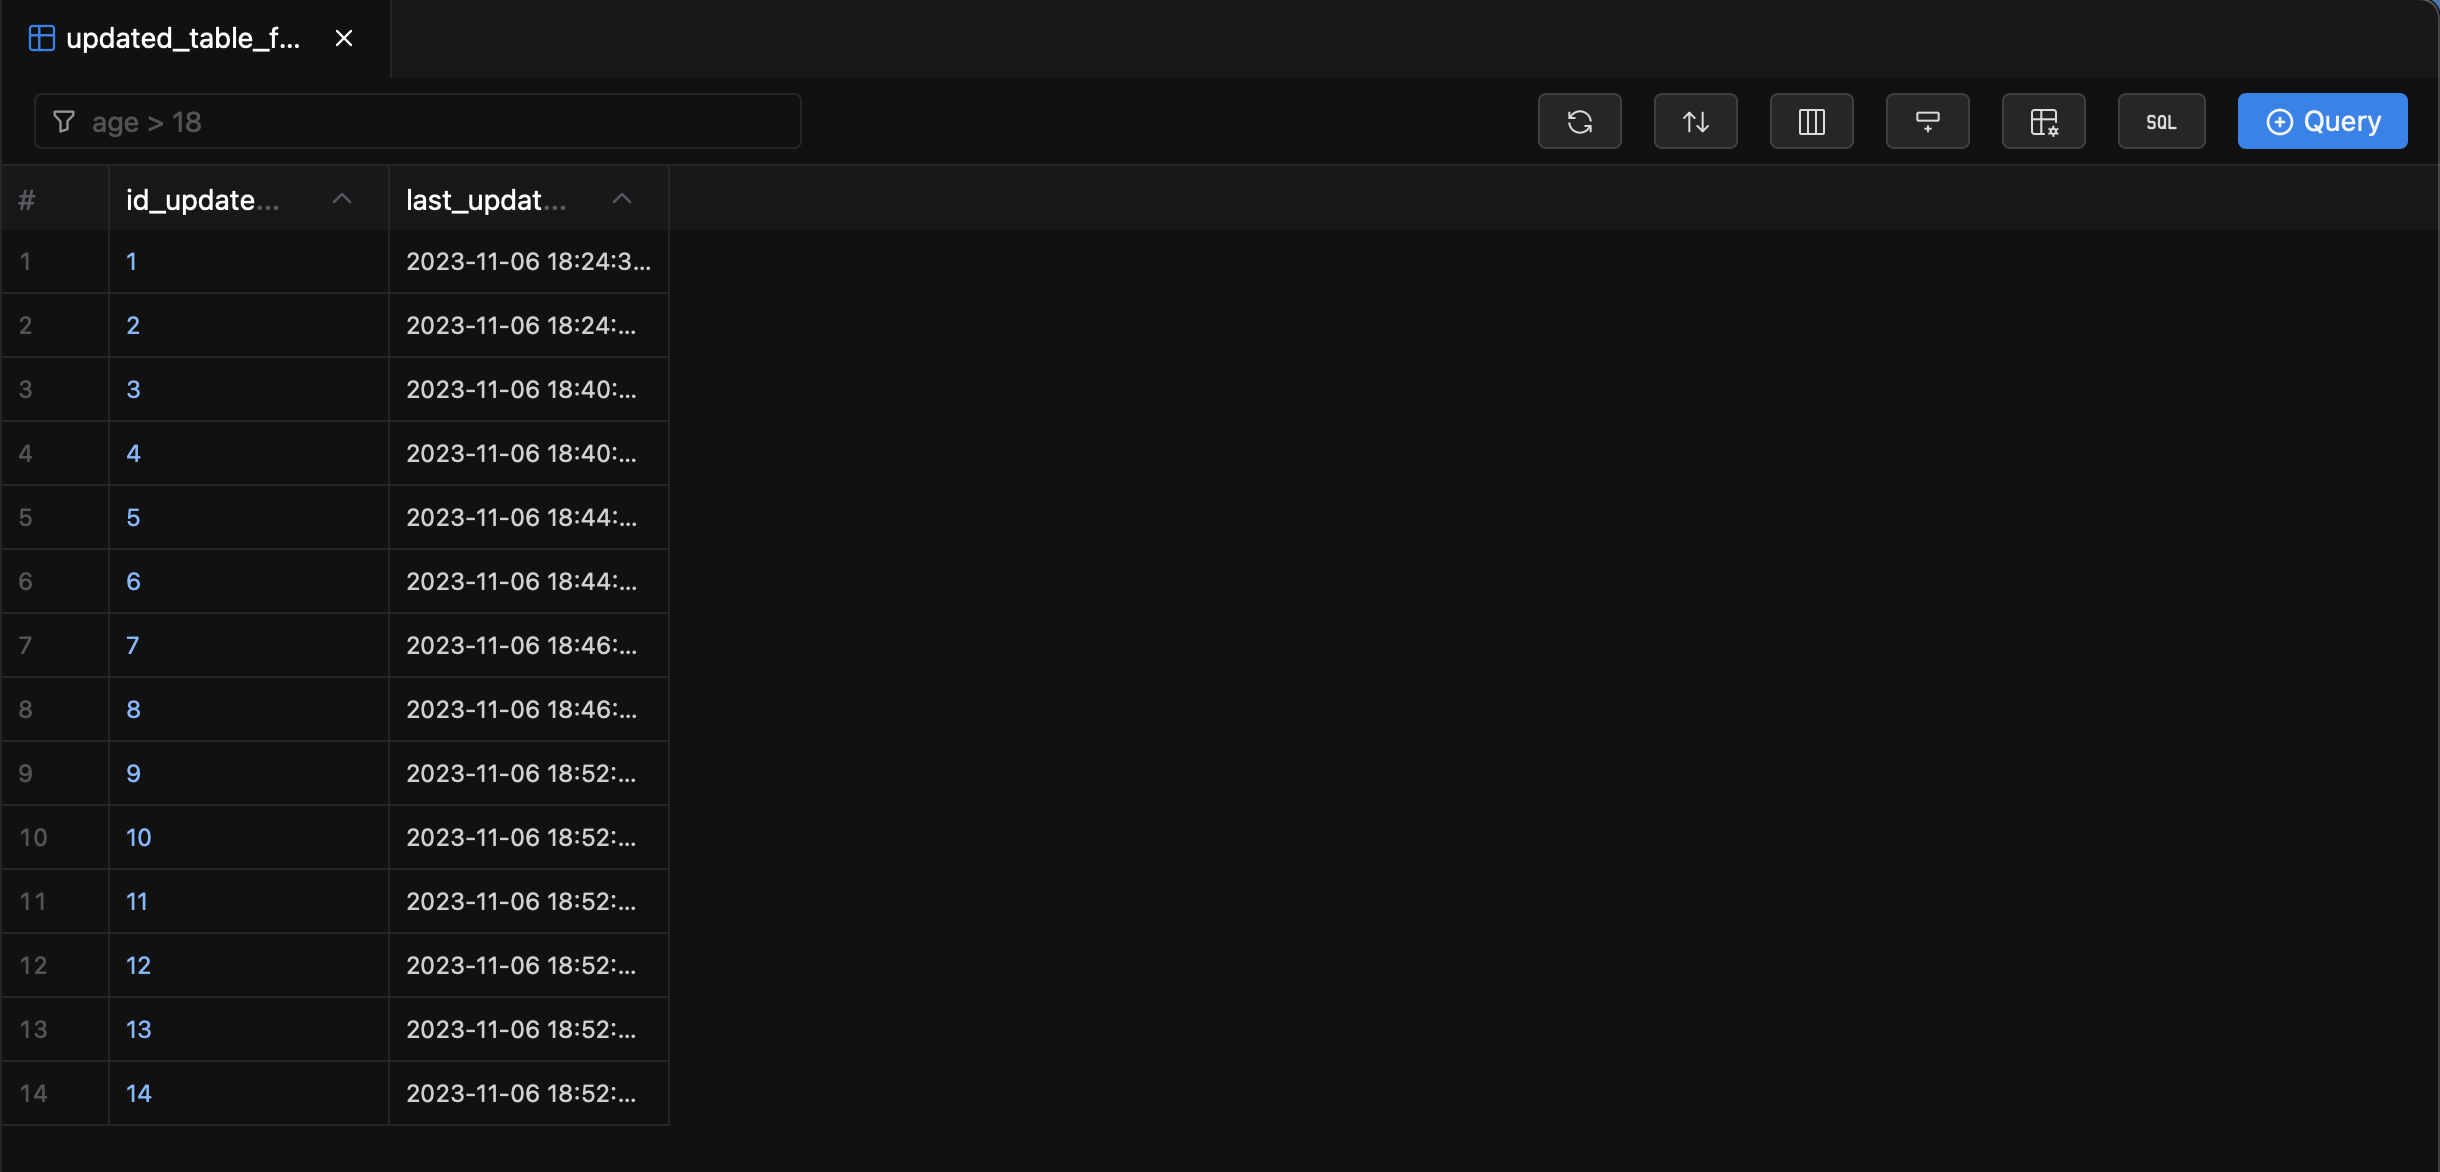
\includegraphics[scale=0.5]{img/Exercice-6-Comprobation.png}
		\caption{Comprobación del funcionamiento del disparador, tabla updated-table-film.}
		\label{fig:Exercice-6}
	\end{figure}

	\section{Ejercicio 8}
	Para este ejercicio se solicita la contrucción de un disparador que guarde en una nueva tabla creada la fecha de cuando se eliminó un registro en la tabla \emph{film}.
\\
	Para la implementación de dicho disparador se ha creado de manera previa una nueva tabla denominada como \emph{deleting-film-rows}, la cual tiene la siguiente estructura:

	\begin{verbatim}
		CREATE TABLE deleting_film_rows (
				delete_id SERIAL PRIMARY KEY,
				film_id INT NOT NULL,
				last_update TIMESTAMP NOT NULL
		);
	\end{verbatim}

	Una vez creada la tabla, se procede a la implementación del disparador, para ello se emplea la siguiente consulta:

	\begin{verbatim}
		-- First we create the function
		CREATE FUNCTION delete_table_film() RETURNS TRIGGER AS $$
				BEGIN
						INSERT INTO deleting_film_rows (film_id, last_update)
						VALUES (OLD.film_id, NOW());
						RETURN OLD;
				END;
		$$ LANGUAGE plpgsql;

		-- Then we create the trigger
		CREATE TRIGGER delete_film_trigger
			AFTER DELETE ON film
			FOR EACH ROW
			EXECUTE PROCEDURE delete_table_film();
	\end{verbatim}

	Comprobación del funcionamiento del disparador \ref{fig:Exercice-7}:

	\begin{figure}[H]
		\centering
		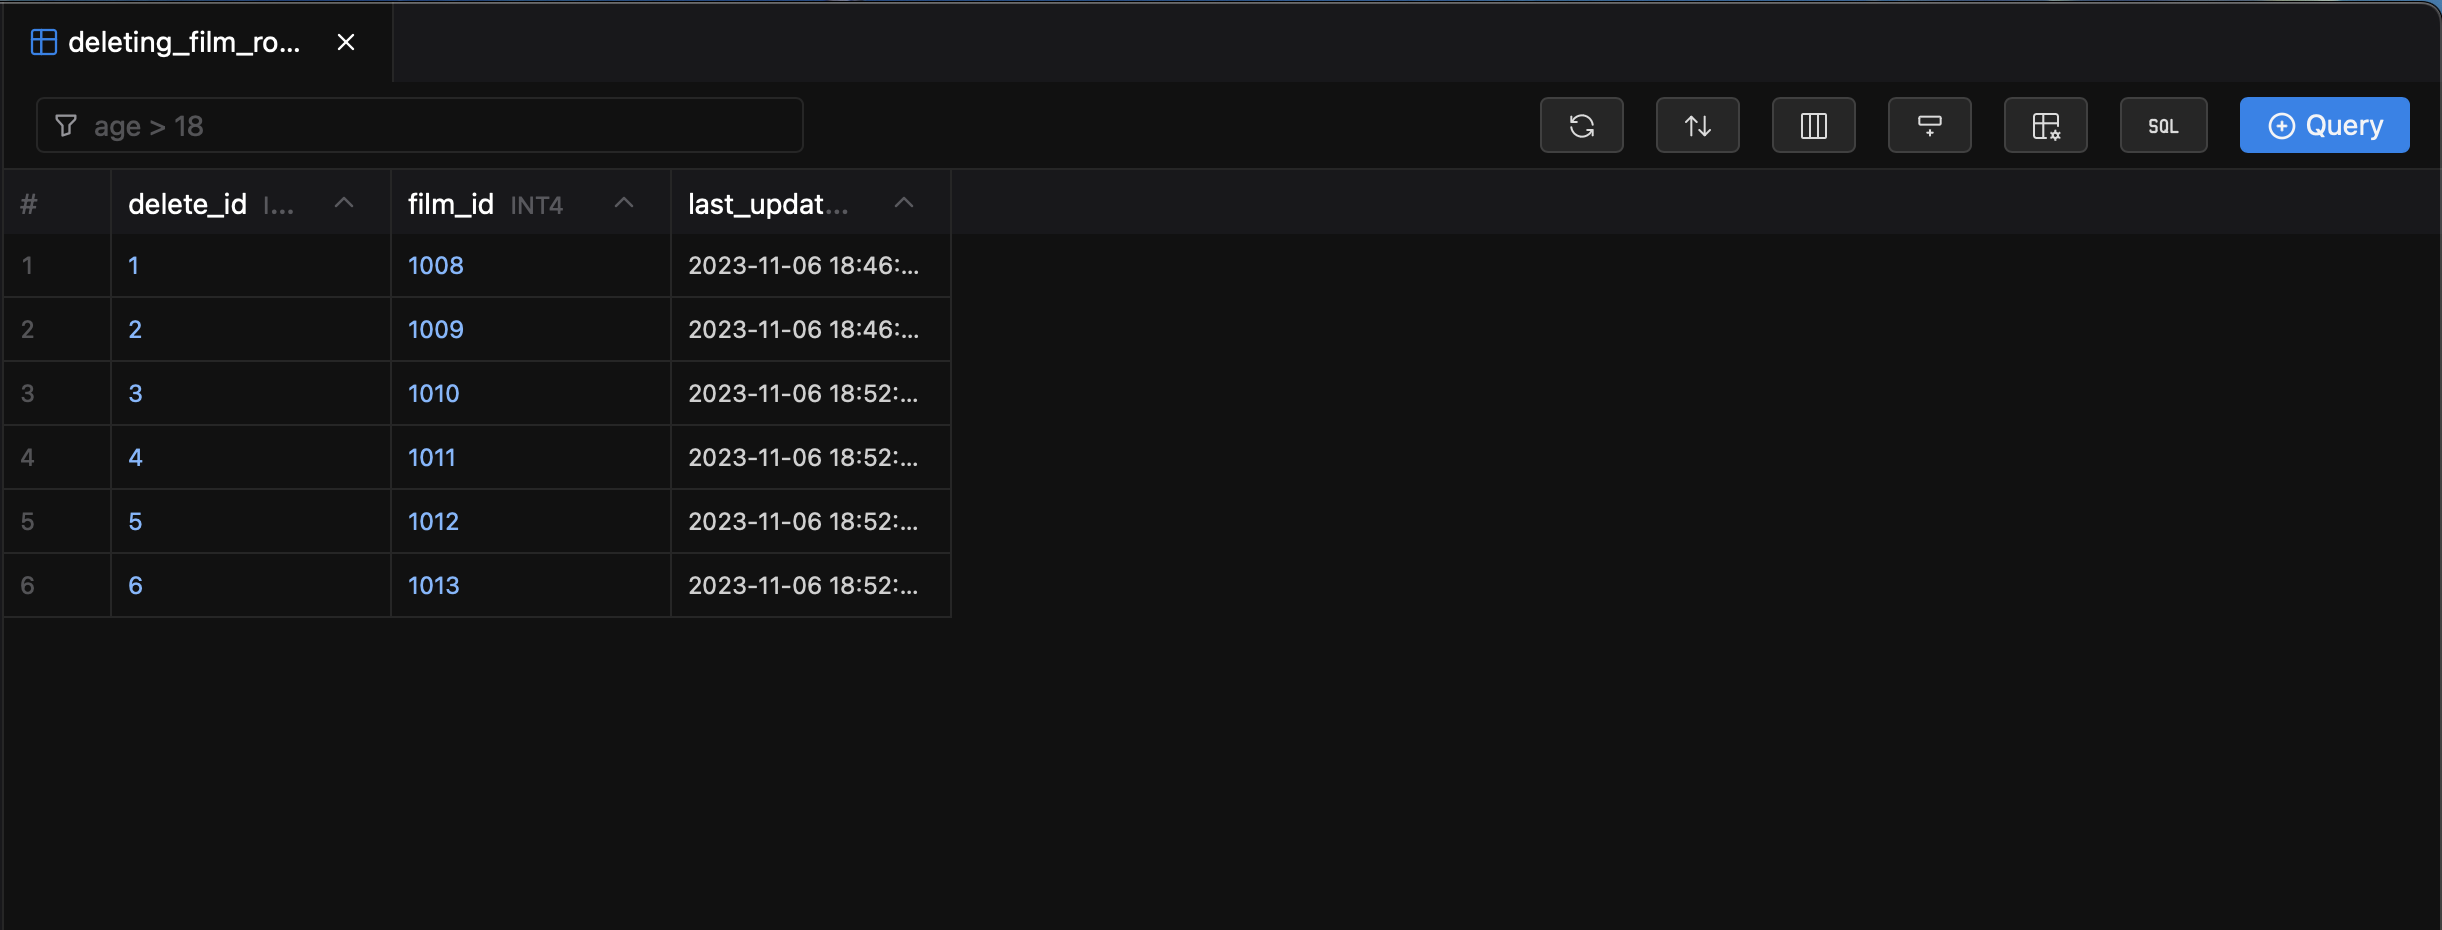
\includegraphics[scale=0.5]{img/Exercice-7-Comprobation.png}
		\caption{Comprobación del funcionamiento del disparador, tabla deleting-film-rows.}
		\label{fig:Exercice-7}
	\end{figure}

	\section{Ejercicio 9}
	Para el octavo y último ejercicio de la práctica se solicita la explicación del término \emph{sequence} y su uso en \emph{PostgreSQL}.
\\
	Es por ello que, las \emph{sequence} en postgresql son objetos que se utilizan para generar valores numéricos de manera secuencial. Estos valores pueden ser utilizados para generar valores de clave primaria o valores de cualquier otra columna.
\\
	Es bastante útil e importante debido a que garantiza la unicidad y la no repetición de valores en una columna, sobre todo importante para el caso de las columnas de clave primaria o identificadores únicos.
\\
	Un ejemplo de creación de una \emph{sequence} en \emph{PostgreSQL} sería el siguiente:

	\begin{verbatim}
		CREATE SEQUENCE nombre_de_la_secuencia START 1 INCREMENT 2;
	\end{verbatim}

	\chapter{Conclusiones}
  Para concluir con esta cuarta práctica de la asignatura \emph{Administración y Diseño de Bases de Datos}, se puede observar que, a pesar de que la base de datos \emph{alquilerdvd} no es muy extensa, se ha podido realizar consultas que permiten obtener información de la misma.
\\
	Es por ello que, gracias a esto se puede prácticar y aprender a realizar consultas de manera correcta y eficiente, de la misma manera en la que se podría realizar en un entorno de trabajo real. Por otro lado, gracias a esto se ha podido comprender la importancia del empleo de triggers que nos permitan realizar aquellas funciones que nosotros queramos dentro de nuestra base de datos, operaciones o funciones como comprobaciones de insersión, eliminación, actualización de elementos dentro de las distintas tablas de nuestra base de datos y operaciones similares. 
\\
	En resumen, esta práctica ha sido fundamental para comprender la importancia de un diseño adecuado de las bases de datos, así como la importancia de su correcta manipulación para obtener resultados precisos y relevantes. Estos conocimientos resultan esenciales para el desarrollo y la administración efectiva de sistemas de bases de datos en entornos reales. 
\\
	\chapter{Bibliografía}
	\begin{enumerate}
		\item OpenAI. (2023). ChatGPT. OpenAI. \url{https://chat.openai.com/}
		\item PostgreSQL. (2023). PostgreSQL: Documentation: 13: CREATE SEQUENCE. PostgreSQL. \url{https://www.postgresql.org/docs/13/sql-createsequence.html}
		\item PostgreSQL. (2023). PostgreSQL: Documentation: 13: CREATE TRIGGER. PostgreSQL. \url{https://www.postgresql.org/docs/13/sql-createtrigger.html}
		\item PostgreSQL. (2023). PostgreSQL: Documentation: 13: CREATE VIEW. PostgreSQL. \url{https://www.postgresql.org/docs/13/sql-createview.html}
		\item PostgreSQL. (2023). PostgreSQL: Documentation: 13: CREATE FUNCTION. PostgreSQL. \url{https://www.postgresql.org/docs/13/sql-createfunction.html}
		\item Samuel Martín Morales. (2023). PostgreSQL-Rent. GitHub. \url{https://github.com/Samuelmm15/PostgreSQL-Rent.git}
	\end{enumerate}	
\end{document}